\documentclass{article}
\usepackage{caption}
\usepackage{algpseudocodex}
\usepackage{algorithm}
\usepackage{amsmath}
\usepackage{xepersian}
\usepackage{graphicx}
\settextfont{XB Niloofar}

\begin{document}
فرض کنید 
$P=\left\{\left(x_1, y_1\right),\ldots, \left(x_n, y_n\right)\right\}$ 
مجموعه‌ای ‌از 
$n$
نقطه در صفحه باشد با این قید که دو یا بیشتر از دو نقطه از آن نقاط روی یک خط عمودی قرار نداشته باشند
و سه یا بیشتر از سه نقطه از آن نقاط روی یک خط قرار نداشته باشند.
 با این فرض، این توصیف متنی از الگوریتمی برای ساخت پوسته‌ محدب مجموعه 
$P$ 
را در نظر بگیرید: 
 
\begin{enumerate}
    \item 
    مجموعه نقاط 
    $P$
    را به ترتیب صعودی مؤلفه 
    $x$
    آنها مرتب کنید تا مجموعه مرتب
    $P'$
    به دست آید. 

    \item 
    پوسته محدب سه نقطه اول در مجموعه مرتب
    $P'$ 
    را که یک مثلث است، 
    بسازید. 

    \item این عملیات را تا زمانی که تمام نقاط مجموعه 
    $P'$ 
    پردازش شوند تکرار کنید: 
    نقطه بعدی در مجموعه 
    $P'$
    را به پوسته محدب فعلی اضافه کنید تا پوسته محدب بزرگ‌تری ایجاد شود. 
    (با اضافه کردن یک نقطه به پوسته فعلی، 
    ممکن است نقاطی که رأسی از پوسته بوده‌اند درون پوسته بعدی قرار گیرند.)


\end{enumerate}

\begin{center}

  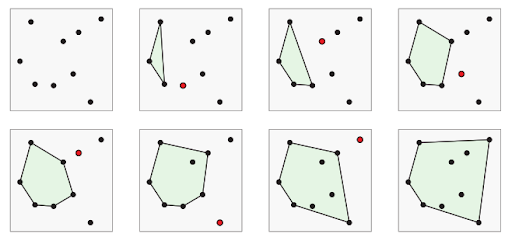
\includegraphics[scale=0.6]{./5_0.png}

\end{center}

\textbf{الف)} الگوریتم را با شبه‌کد آنقدر دقیق توصیف کنید که بتوان به راحتی
 مبتنی بر آن شبه‌کد، برنامه‌ای برای پیاده‌سازی الگوریتم نوشت.
 توصیف دقیق الگوریتم، مستلزم آن است که مشخص کنیم در هر مرحله،
 نقطه بعدی در لیست مرتب نقاط به کدام یک از دو نقطه پوسته محدب فعلی وصل می‌شود.

\textbf{ب)}
الگوریتم را چگونه باید غنی کرد تا در حالاتی هم که دو یا بیشتر از دو نقطه روی یک خط عمودی قرار داشته باشند، درست کار کند؟
الگوریتم را چگونه باید غنی کرد تا در حالاتی هم که سه یا بیشتر از سه نقطه روی یک خط قرار داشته باشند، درست کار کند؟  

\textbf{پ)}
ثابت کنید که می‌توان کارایی زمانی الگوریتم برای ساخت پوسته محدب هر مجموعه
$n$
  نقطه‌ای را به صورت 
  $O(n^2)$
  بیان کرد. 

\end{document}